\documentclass[12pt]{article}

% Opening
\title{Math 3012 Final Exam Part A}
\author{Akash Narayanan}

\usepackage{amsmath, amsfonts, amssymb, amsthm, enumitem, tikz}
\usepackage{caption, subcaption, float, marginnote, mathtools, mdframed}

% Solution environment
\newenvironment{solution}{
\begin{mdframed}
  { {\bfseries Solution}: }}{
\end{mdframed}}

\begin{document}

  \maketitle

  \begin{enumerate}

    % Problem 1
    \item (20 points)
    \begin{enumerate}[label=({\alph*})]
      \item (10 points) Use the Euclidean algorithm to find \(d = \text{gcd}(115, 161)\).

      \item (10 points) Use your work in the preceding problem to find integers \(a\) and \(b\) so that \(d = 115a + 161b\).
    \end{enumerate}

    \begin{solution}
      \begin{enumerate}[label=({\alph*})]
        \item We use the Euclidean algorithm to find \(d\):
        \begin{align*}
          161 &= 1 \cdot 115 + 46 \\
          115 &= 2 \cdot 46  + 23 \\
          46  &= 2 \cdot 23  + 0  \\
          d &= 23
        \end{align*}
        So \(\text{gcd}(115, 161) = 23\)

        \item We use the extended Euclidean algorithm to find \(a\) and \(b\):
        \begin{align*}
          23 &= 115 - 2 \cdot 46 \\
             &= 115 - 2 \cdot (161 - 1 \cdot 115) \\
             &= 3 \cdot 115 - 2 \cdot 161
        \end{align*}
        Thus, \(a = 3\) and \(b = -2\)
    \end{enumerate}
    \end{solution}

    \pagebreak

    % Problem 2
    \item (20 points)
    \begin{enumerate}[label=({\alph*})]
      \item (10 points) For a positive integer \(n\), let \(q_{n}\) count the number of quaternary string (\(\text{alphabet} = \{0, 1, 2, 3\}\)) that do not contain either 11 or 002 as substrings of consecutive characters.
      Find initial conditions by specifying \(q_{1}\), \(q_{2}\), and \(q_{3}\).

      \item (10 points) Develop a recurrence for \(q_{n}\) when \(n \geq 4\) and use it to compute \(q_{4}\) and \(q_{5}\).
    \end{enumerate}

    \begin{solution}
      \begin{enumerate}[label=({\alph*})]
        \item Clearly \(q_{1} = 4\) since there are 4 possible strings of length 1, none of which contain the disallowed substrings.
        \(q_{2}\) is found by considering all strings of length 2, of which there are \(4^{2} = 16\). Only one contains the substring 11, so \(q_{2} = 15\).
        For \(q_{3}\), start by considering all strings of length 3. There are \(4^{3} = 64\). Only one contains the substring \(002\). There are 7 containing the substring 11, namely those of the form \(11x\) and \(x11\) where \(x\) is 0, 2, or 3, along with 111. Thus, \(q_{3} = 56\).

        \item Given \(q_{n-1}\), there are \(4 q_{n-1}\) strings that can be formed by appending one letter from the alphabet to the end of each valid string of length \(n-1\).
        We count the number of bad strings formed this way. The number of strings  of length \(n\) ending in "002" must be equal to the number of good strings of length \(n - 1\) ending in "00" (the two are in bijection).
        Similarly, the number of good strings of length \(n - 1\) ending in "00" is equal to the number of good strings of length \(n - 2\) ending in "0" which is equal to the number of good strings of length \(n - 3\), or \(q_{n - 3}\).

        Using a similar line of reasoning, a string ending with 1 is bad if the first \(n - 2\) characters are valid and the \((n - 1)\)-th character is a 1.
        However, this implies the string of length \(n - 2\) must not end with a 1, further implying that the string of length \(n - 3\) must not end with a 1.
        Thus, there are 3 options for the last character of the corresponding valid string of length \(n - 3\).

        Thus, our recurrence relation is
        \begin{equation*}
          q_{n} = 4 q_{n - 1} - q_{n - 2} - q_{n - 3} + 3 q_{n - 4}
        \end{equation*}
        We find that \(q_{4} = 208\) and \(q_{5} = 773\).
      \end{enumerate}
    \end{solution}

    \pagebreak

    % Problem 3
    \item (20 points) Consider the following network flow:

    \begin{figure}[H]
      \begin{center}
        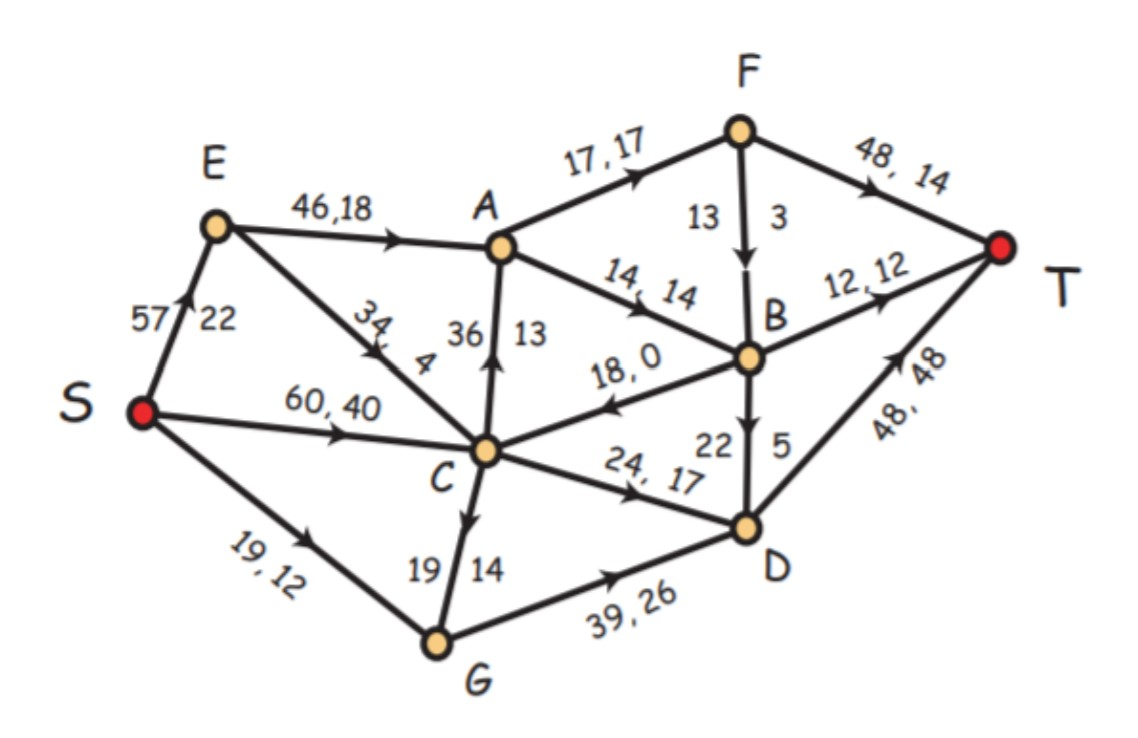
\includegraphics[width=0.8\textwidth]{media/Network Flow Final.jpg}
      \end{center}
    \end{figure}

    \begin{enumerate}[label=({\alph*})]
      \item (7 points) The value of the current flow is:

      \item (7 points) The capacity of the cut \(\{S, B, D, E, G\} \cup \{A, C, F, T\}\) is:

      \item (6 points) Carry out the labeling algorithm, using the pseudo-alphabetic order on the vertices and list below the labels which will be given to the vertices.
    \end{enumerate}

    \begin{solution}
      \begin{enumerate}[label=({\alph*})]
        \item The value of the current flow is the total flow leaving the source, which is \(22 + 40 + 12 = 74\).

        \item The capacity of the cut is the sum of the capacities over edges moving from the set with the source to the st with the sink.
        The forward edges are SC, BT, BC, DT, EA, and EC.
        Thus, the capactiy of the cut is \(60 + 12 + 18 + 48 + 46 + 34 = 218\).

        \item We use the Ford-Fulkerson algorithm
        \begin{center}
          \begin{tabular}{c c}
            Vertex & Label \\
            S & (*, +, \(\infty\)) \\
            C & (S, +, 20) \\
            E & (S, +, 35) \\
            G & (S, +, 7) \\
            A & (C, +, 20) \\
            D & (C, +, 7) \\
            B & (D, -, 5) \\
            F & (B, -, 3) \\
            T & (F, +, 3) \\
          \end{tabular}
        \end{center}
        The algorithm did not halt so the given flow is not maximal. It can be repeated until it does halt in order to find a maximal flow.
      \end{enumerate}
    \end{solution}

    \pagebreak

    % Problem 4
    \item (20 points) Show that the graph below is Hamiltonian. You may give your answer by darkening appropriate edges on the figure, or by giving an appropriate permutation of the vertex set.

    \begin{figure}[H]
      \centering
      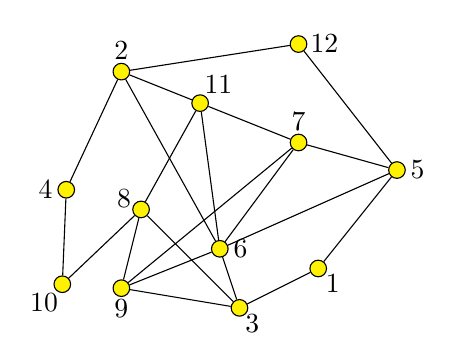
\begin{tikzpicture}
        [scale=1,every node/.style={draw,shape=circle,fill=yellow,inner sep=0,minimum size=6pt}, every draw/.style={line width=0.25mm, black}]

        \node[label=315:{1}] (v1) at (-.5, -0.5) {};
        \node[label=90:{2}] (v2) at (-3, 2) {};
        \node[label=300:{3}] (v3) at (-1.5, -1) {};
        \node[label=180:{4}] (v4) at (-3.7, 0.5) {};
        \node[label=0:{5}] (v5) at (0.5, 0.75) {};
        \node[label=0:{6}] (v6) at (-1.75, -0.25) {};
        \node[label=90:{7}] (v7) at (-0.75, 1.1) {};
        \node[label=165:{8}] (v8) at (-2.75, 0.25) {};
        \node[label=270:{9}] (v9) at (-3, -0.75) {};
        \node[label=225:{10}] (v10) at (-3.75, -0.70) {};
        \node[label=45:{11}] (v11) at (-2, 1.6) {};
        \node[label=0:{12}] (v12) at (-0.75, 2.35) {};

        \draw (v1) -- (v3);
        \draw (v1) -- (v5);
        \draw (v2) -- (v4);
        \draw (v2) -- (v6);
        \draw (v2) -- (v11);
        \draw (v2) -- (v12);
        \draw (v3) -- (v6);
        \draw (v3) -- (v8);
        \draw (v3) -- (v9);
        \draw (v4) -- (v10);
        \draw (v5) -- (v6);
        \draw (v5) -- (v7);
        \draw (v5) -- (v12);
        \draw (v6) -- (v7);
        \draw (v6) -- (v9);
        \draw (v6) -- (v11);
        \draw (v7) -- (v9);
        \draw (v7) -- (v11);
        \draw (v8) -- (v9);
        \draw (v8) -- (v10);
        \draw (v8) -- (v11);
      \end{tikzpicture}
    \end{figure}

    \begin{solution}
      A Hamiltonian cycle for this graph is (10, 4, 2, 12, 5, 1, 3, 9, 6, 7, 11, 8). A visualization of this cycle is shown below.

      \begin{figure}[H]
        \centering
        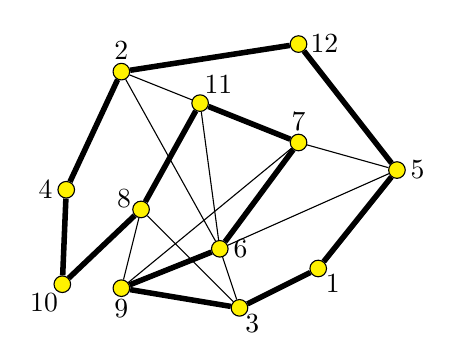
\begin{tikzpicture}
          [scale=1,every node/.style={draw,shape=circle,fill=yellow,inner sep=0,minimum size=6pt}, every draw/.style={line width=0.25mm, black}]

          \node[label=315:{1}] (v1) at (-.5, -0.5) {};
          \node[label=90:{2}] (v2) at (-3, 2) {};
          \node[label=300:{3}] (v3) at (-1.5, -1) {};
          \node[label=180:{4}] (v4) at (-3.7, 0.5) {};
          \node[label=0:{5}] (v5) at (0.5, 0.75) {};
          \node[label=0:{6}] (v6) at (-1.75, -0.25) {};
          \node[label=90:{7}] (v7) at (-0.75, 1.1) {};
          \node[label=165:{8}] (v8) at (-2.75, 0.25) {};
          \node[label=270:{9}] (v9) at (-3, -0.75) {};
          \node[label=225:{10}] (v10) at (-3.75, -0.70) {};
          \node[label=45:{11}] (v11) at (-2, 1.6) {};
          \node[label=0:{12}] (v12) at (-0.75, 2.35) {};

          \draw (v1)[line width = 2] -- (v3);
          \draw (v1)[line width = 2] -- (v5);
          \draw (v2)[line width = 2] -- (v4);
          \draw (v2) -- (v6);
          \draw (v2) -- (v11);
          \draw (v2)[line width = 2] -- (v12);
          \draw (v3) -- (v6);
          \draw (v3) -- (v8);
          \draw (v3)[line width = 2] -- (v9);
          \draw[line width = 2] (v4) -- (v10);
          \draw (v5) -- (v6);
          \draw (v5) -- (v7);
          \draw (v5)[line width = 2] -- (v12);
          \draw (v6)[line width = 2] -- (v7);
          \draw (v6)[line width = 2] -- (v9);
          \draw (v6) -- (v11);
          \draw (v7) -- (v9);
          \draw (v7)[line width = 2] -- (v11);
          \draw (v8) -- (v9);
          \draw (v8)[line width = 2] -- (v10);
          \draw (v8)[line width = 2] -- (v11);

        \end{tikzpicture}

      \end{figure}
    \end{solution}

    \pagebreak

    % Problem 5
    \item (20 points) Is the binary relation
    \begin{equation*}
      P = \{(1, 1), (2, 2), (3, 3), (4, 4), (1, 3), (2, 4), (3, 4)\}
    \end{equation*}
    a partial order on the set \(X = \{1, 2, 3, 4\}\)? If so, discuss what properties you verified and how. If not, list the ordered pairs that must be added to \(P\) to make it a partial order, in case it is possible.

    \begin{solution}
      A partial order is reflexive, antisymmetric, and transitive. The given relation is reflexive and antisymmetric.
      However, it is not transitive since \((1, 3) \in P\) and \((3, 4) \in P\), but \((1, 4) \notin P\).
      Thus, by adding \((1, 4)\) to \(P\) we make it a partial order.
    \end{solution}
  \end{enumerate}
\end{document}
